\documentclass[../../main.tex]{subfiles}

%academic year.  
%
%(a) Armed Services and Govt. Internships, Andrew Householder, Natasha Waldorf, Adam Wildanger, Dane Goodman (volunteering) (b) Ondrasik-Groce Fellowship, Raymond Hartig (c) WSP and Jackson Diamond, and future COSC+WSP connections (d) Matthew Buchanan Garza, and the IDC grant for PhET creation (e) advising and mentoring first years.
%
%If i was so rigid in my advising, why would I encourage folks to join WSP?  WSP is all about thinking productively about a topic from multiple perspectives, creating a path for your own future through development of the educational process, and independently executing an original idea. 
%
%Why not LinkedIn?  In our discussions of a new curriculum, we propose to ask them to create a digital portfolio of projects they can later present future colleagues.  How is this different?
%
%I literally said this ``Sometimes the interests of the student align with my research, and sometimes they do not. I
%advise them nonetheless, and do my best to meet the student where they are to guide them forward.'' And yet you somehow arrived at the conclusion that my practice is too rigid.  Go figure.
%
%Did you not understand the story of my advisee Wyatt?  We literally changed his major from STEM to humanities and he felt that it was the right path.
% 
\begin{document}
\label{sec:advising_mentoring}

I reflect in this section on my role as an advisor and mentor.  On my role as an academic advisor, I highlight four themes in my reflections below.  (1) My ongoing participation in the Whittier Scholars Program is evidence that I am committed to interdisciplinary studies and the liberal arts.  (2) I have shown concrete examples of helping students broadening their vision to include new disciplines.  (3) The proportion of my students selecting ICS/Math and ICS/Physics continues to increase.  (4) According to the self-study completed by my department, I am responsible for a large portion of the first-year advising work my department contributes to the college.  It will be wise to rebalance that work, so I will likely reduce my first-year advising in the short term and increase advising of physical science and WSP majors.
\\
\vspace{0.25cm}
In Tab. \ref{tab:advisees}, I summarize my advisees within the first-year orientation program, physical sciences, and Whittier Scholars Program.  After each entry, I indicate the outcome after their time at Whittier College, or their current job, or their plans upon graduation.  I have included my students in Physics Research (PHYS396), which is a course my department maintains to provide students 1-3 credits for doing research with us.  Though these credits do not count towards my teaching load, I provide these opportunities so that students can participate in my research and deepen their scientific and engineering toolkits.

\begin{table}[hb]
\small
\centering
\begin{tabular}{| c | c | c |}
\hline
\hline
Semester & \textbf{Number of First Year Advisees} & Note/Outcome \\ \hline
Fall 2019 & 15 & I taught physics \\ \hline
Fall 2020 & 14 & I taught INTD100 \\ \hline
Fall 2022 & 13 & I am teaching INTD100 \\ \hline
\hline
All semesters & \textbf{Physics, ICS, and 3-2 Majors} & \\ \hline 
& Cassady Smith (Physics '20) & Graduate student at Yale Univ., Keck Fellowship \\ \hline
& John Paul G\'{o}mez-Reed (Math/ICS '21) & Keck Fellow, Ondrasik-Groce Fellow \\ \hline
& Nicolas Clarizio (Physics, Business Admin. '19) & Mechanical Engineer, SMP Engineering Inc. \\ \hline
& Alex Ortiz-Valenzuela (3-2 Engineering/Physics  '22) & Admitted to Cal Poly Pomona, 3-2 program \\ \hline
& Raymond Hartig (Physics and Math '23) & Ondrasik-Groce Fellow, Fletcher-Jones Fellow \\ \hline
& Adam Wildanger (3-2 Engineering/Physics '21) & Admitted to USC, 3-2 program \\ \hline
& Matthew Buchanan Garza (ICS/Physics '23) & Working on DEI project (Sec. \ref{sec:dei}) \\ \hline
& Natasha Waldorf (ICS/Physics '24) & Currently at AFRL internship \\ \hline
& Dane Goodman (Physics with Math Minor '23) & Volunteering in my ONR projects \\ \hline \hline
All semesters & \textbf{Whittier Scholars Program Majors} & \\ \hline
& Nicolas Bakken-French (WSP '21) & Publishing book on glaciology and culture \\ \hline
& Jackson Diamond (WSP '23) & Developing bluetooth positioning system \\ \hline \hline
Current Semster & \textbf{PHYS396 Students}  & \\ \hline
& Matthew Buchanan Garza (ICS/Physics '23) & Working on DEI project (Sec. \ref{sec:dei}) \\ \hline
& Jackson Diamond (WSP '23) & Developing bluetooth positioning system \\ \hline
& Dane Goodman (Physics with Math Minor '23) & Volunteering in my ONR projects \\ \hline
& Raymond Hartig (Physics and Math '23) & Ondrasik-Groce Fellow, Fletcher-Jones Fellow \\ \hline
& Alex Ortiz-Valenzuela (3-2 Engineering/Physics '22) & Admitted to Cal Poly Pomona, 3-2 program \\ \hline
& Riley Sullivan (Physics '23) & Continuing Askaryan radiation research \\ \hline
& Ian Watanabe (ICS/Physics '23) & Continuing Askaryan radiation research \\ \hline
& Natasha Waldorf (ICS/Physics '24) & Currently at AFRL internship \\ \hline
\end{tabular}
\caption{\label{tab:advisees} A summary of my advisees, broken into three categories: first-year advisees, STEM majors, and WSP majors.  There are some first year advisees who have chosen ICS/Math for their major, for whom I remain a mentor.  One example is Emily List (ICS/Math '23).  Listed in the lower portion of the table are my PHYS396 - Physics Research students.}
\end{table}

\section{Advising First Year Students}

Reflecting on my time advising first-year students, I realize the first-year orientation and advising process has evolved substantially since I arrived in 2017.  During my second year serving the Enrollment and Student Affairs Committee (ESAC) with Prof. Gil Gonzalez, we discussed the INTD101 pilot program and I learned more about INTD100 and first-year orientation from Prof. Lagan.  Since Prof. Gonzalez has now fully implemented the INTD101 program, the orientation side of the process has been standardized, with course and curricular advising left to the professors.  I find it easier to understand my role within the new system.  It allows me more time to focus on the academics of my students, leaving orientation to campus to staff colleagues in CAAS, Wardman Library, and INTD101 content.  
\\
\vspace{0.25cm}
Most of my first-year students decide upon a major program before arriving.  Because I am in the physical sciences, the system steers to me students who have declared a physical science major.  Occasionally, I encounter someone who is open to exploring programs before choosing a major.  When I encounter someone who is genuinely open, I first ask myself if Whittier Scholars is right for them.  The students I have encountered who thrive in WSP have a self-determination and willingness to act on their instincts.  Though I wish all of our students had these qualities, the added responsibility intrinsic to WSP is not for everyone.  We want our WSP advisees to genuinely take charge of the educational design, and think strategically about coursework and internships.  Some of my first year students simply want to begin a pre-designed major that suits their interests.  That being said, I do maintain a committment to the liberal arts and to interdisciplinary studies via WSP and advising.
\\
\vspace{0.25cm}
As evidence for this, I included the example of my student Wyatt Killien in my prior PEGP report (Secs. 5.1 and 5.2).  In our last communication you shared a concern that my advising is too ``rigid.''  I understand that to mean you do not want me to guide students down a pre-determined path, but foster a sense of exploration in areas other than STEM.  Usually, the orientation organizers direct first-year students interested in STEM subjects to me.  I do have the ability to recognize when a student needs to explore outside their initial plan.  Wyatt is a student who listed physics as the choice of major, but I detected that Wyatt was off-course after a few meetings.  I knew right away that WSP would not be a good fit, because the student works a full-time job and prefers the structure associated with a pre-defined major.  The interest the student has in physics does not extend to the scientific mindset, but is more focused on the \textit{order} with which physics describes the Universe.  Wyatt is someone who is interested in science fiction, art and design, and manga and anime.  I recommended 100-level art and design courses, and Wyatt joined them with enthusiasm and later changed his major.  
\\
\vspace{0.25cm}
I have engaged in other advising moments with first-year students that caused them to expand their horizons, even if it did not benefit me or my department.  Recall that I taught a CON2 course INTD255 entitled ``Safe Return Doubtful: History and Current Status of Modern Science in Antarctica.''  Sophie Frizzell was my student in INTD255.  Sophie excitedly informed me in class this semester of her new career path in wildlife conservation after experiencing my teaching in INTD255.  Sophie has been working with an organization that protects and reintroduces infant elephant seals in Northern California.  INTD255 was heavily laden with lessons meant to inspire students to actively chart their own course as explorers.  Sophie is an example of a student who, after interacting with me, actively adjusted their educational trajectory to explore new worlds.  Another example of a student inspired by my teaching in a CON2 course is Scout Mucher, who recently graduated from Whittier College after taking my INTD290 course entitled ``History of Science in Latin America.''  After consultation with me, Scout decided to actually journey to Antarctica to work as a contractor to run McMurdo Station, the primary base of the United States Antarctic Program (USAP).  To quote from my prior PEGP:

\begin{quotation}
Sometimes the interests of the student align with my research, and sometimes they do not. I advise them nonetheless, and do my best to meet the student where they are to guide them forward.
\end{quotation}

\section{Advising and Mentoring Majors in Physics, ICS, and 3-2 Engineering}

My upper-division advisees plan to major in one of three areas: Physics, ICS, or 3-2 Engineering.  In our last communication, I shared a logical framework that informs my advising with these students in the form of a decision tree.  You shared a concern about the tree, and concerns that the use of social media tools like LinkedIn does not always help these students.
\\
\vspace{0.25cm}
In our last communication, I do not think I made it clear that the structure of Fig. \ref{fig:tree} is not something I thrust upon the students.  The division of the pathway after college into three branches is a cultural phenomenon for undergraduate students in the physical sciences.  The classifications of academia, public sector, and private sector are commonly discussed.  For the latter, sometimes students use the term ``industry,'' as in, ``I'm going into industry'' (in my field).  When I use this classification (the top-level of Fig. \ref{fig:tree}), I am mirroring the language the students use with each other.  Beneath the three-part classification of the utility of a degree in the physical sciences I have added common examples of ways in which Whittier graduates might serve.
\\
\vspace{0.25cm}
For example, if a student is determined to stay on the academic track, and is a double major in physics and mathematics, graduate school is the logical choice.  My long-time advisee and friend Raymond Hartig is pursuing this path, for example.  I do not \textit{require} my students who pursue this pathway stay on this pathway.  Students often drift from their initial choice to a choice that better matches their situation.  Graduate school, as you well know, is a large investment of time.  Some students discover they would rather spend that time on starting a family or at a more lucrative job in the private sector.  The advisee listing in Tab. \ref{tab:advisees} shows that a large majority of my students do not wish to pursue graduate studies in physics or math.  What has become increasingly common for my advisees that do remain in the Physics/ICS/3-2 area is to choose the ICS/Math major with the intention of going into software development and machine learning.
\\
\vspace{0.25cm}
This increase in ICS enrollment, which began in 2018, has been modified in two ways.  First, some \textit{physics} students are now choosing to double-major in ICS/Physics and Physics, taking advantage of the overlap in courses\footnote{I have not yet encountered a double major in ICS/Math and Physics, which would be much more challenging but very interesting.}.  This choice keeps both the academic physics track and private sector software options open, and it also enhances their skill in computational physics\footnote{See the discussion about CEM in Sec. \ref{sec:scholarship}.}.  I teach these students personally in Computer Logic and Digital Circuit Design (COSC330/PHYS306).  For this reason, I feel this course needs to include more machine learning topics in its next upgrade.  The second way in which ICS enrollment has changed is that more first-year students are arriving without the pre-requisite math skills.

\begin{figure}[hb]
\centering
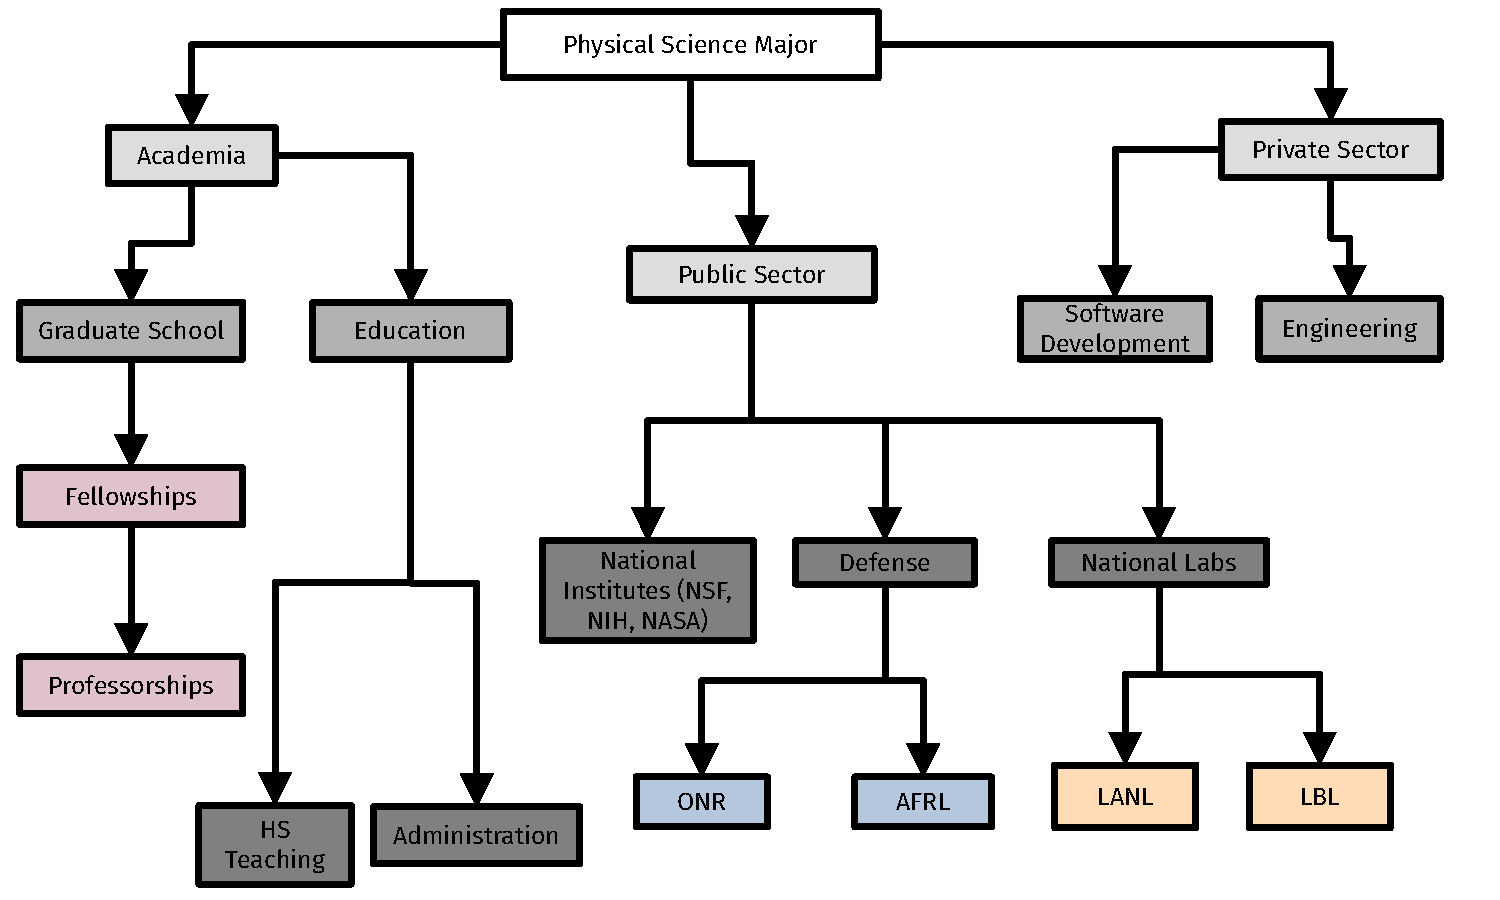
\includegraphics[width=0.65\textwidth]{figures/tree.pdf}
\caption{\label{fig:tree}}
\end{figure}

The ICS core course list includes the standard three-semester sequence of calculus courses.  Students who start at MATH085 or below are automatically delayed a semester in completing the ICS core.  I have begun to observe this effect in my advisees this year, some of whom are unable to begin with MATH141 (Calculus 1) because of their Math Placement Exam score, or because they did not take IB or AP Calculus in high school.  One of my advisees claims to be qualified to take Calculus 1, but did not receive a 4 on the Math Placement Exam.  The student is an international student who passed IB courses.  As part of the QSC director search, my colleagues have shared anecdotal evidence that math preparation suffered during the online learning period of the pandemic, but grades and test scores received in high school remained constant.  As I begin to take on more ICS/Math and ICS/Physics majors, I will have to watch for this situation and help my students plan accordingly.  In the long term, I hope the QSC will help accelerate this trajectory for our students.
\\
\vspace{0.25cm}
I really enjoy mentoring ICS, Physics and 3-2 majors, and my research with them has inspired them to excel (see Note/Outcome in Tab. \ref{tab:advisees}).  However, the vast majority of my advisees have been first-years.  In the next few years, it will be wise to reduce my first-year advising load to focus on 3-2, ICS, and Physics majors, for two reasons.  First, according to our department self-study, I provide the majority of the INTD100 and first-year advisee contributions from my department.  Our most recent self-study acknowledged that this is unbalanced and will be rectified in the coming semesters.  Second, I have not taught our senior seminar course, PHYS499, and I usually have only 1-2 advisees per year who graduate in 3-2, ICS, or Physics.  There are cases like Andrew Householder (ICS/Physics and Physics '23, private sector track), who have performed ample \textit{research} with me, but do not appear in Tab. \ref{tab:advisees} because they are not my \textit{advisees.}  I helped Andrew secure an internship at The Aerospace Corporation this past Summer (private track in Fig. \ref{fig:tree}).  The bottom line is my involvement with our graduating majors should increase.  I have worked closely with Raymond Hartig (academic track) for two years, and Raymond plans to attend graduate school for physics.
\\
\vspace{0.25cm}
Others in my group of major advisees have chosen the public sector track.  For example, Natasha Waldorf took her cue from my Computer Logic and Digital Circuit Design course.  Within that course, I promoted public sector internship opportunities with the US Navy (NREIP and SMART scholarships) and the Air Force.  With the remote research experiences I provided as a starting point, Natasha went on to land an Air Force Research Laboratory (AFRL) Summer internship near New Mexico State University.  Natasha was offered a full-time job with AFRL before the start of the Fall 2022 semester.  We met regularly on Discord to strategize, and we ultimately decided that Natasha would be a part-time student at Whittier College to gain the experience and income.  The goal for Natasha is to get involved with low Earth-orbit satellite deployment, integrating intelligence, agricultural, and weather data from our fleet of satellites.
\\
\vspace{0.25cm}
I include this example because it shows that I advise students along all three main branches in Fig. \ref{fig:tree} (public sector, private sector, and academic track).  In my view, the wise strategy is to support the student by sharing knowledge and by motivating them while leaving the key decisions in their hands.  I believe that it is morally wrong to ``steer'' students in directions that serve our interests, or to claim that we know better than the student or the family of the student what path is most appropriate.  In the essay \textit{Solitude and Leadership}, William Deresiewicz argued (in front of thousands of graduates of West Point) \cite{west_point} that good leadership means learning to lead yourself first in solitude and then to think for yourself creatively.  I share this essay in all my non-physics courses.  We must lay out the path for our student, and ask them to take the time to organize their own thinking and to have the moral courage to act on their best judgement.  Students who do not do this tend to ``go with the flow,'' taking courses and choosing majors based on vague or practical reasoning.  I submit to you that students who perform this self-reflection thrive in liberal arts institutions, because we provide many diverse pathways to graduation and we pride ourselves on honing their ability to think about the big picture.

\section{Advising and Mentoring Whittier Scholars Program Majors}

Things.

\end{document}
